\documentclass[11pt]{exam}

\usepackage{amsmath}
\usepackage{graphicx}
\usepackage{geometry}
\usepackage{etoolbox}
\BeforeBeginEnvironment{choices}{\par\nopagebreak\minipage{\linewidth}}
\AfterEndEnvironment{choices}{\endminipage}
\geometry{
a4paper,
total={185mm,257mm},
left=10mm,
top=25mm,
bottom=10mm
}

\begin{document}
\setlength{\voffset}{-0.5in}
\setlength{\headsep}{5pt}

\fbox{\fbox{\parbox{8cm}{\centering
\vspace{2mm}
Testat - Versuch K - Radioaktivitaet - 3
\vspace{2mm}
}}}
\hspace{2mm}
\makebox[0.25\textwidth]{Name:\enspace\hrulefill} \hspace{5mm}
\makebox[0.2\textwidth]{Datum:\enspace\hrulefill}
\vspace{4mm}

\begin{questions}

\question Die Aktivität einer radioaktiven Substanz wird in Becquerel angegeben. Wie setzt sich diese Größe aus den  SI-Basiseinheiten zusammen?

\begin{choices}
	\choice \( \text{s}^{-1} \)
	\choice \( \text{kg}\cdot\frac{\text{m}}{\text{s}^2} \)
	\choice \( \frac{\text{J}}{\text{kg}} \)
	\choice \( \frac{\text{J}}{\text{s}} \)
	\choice s
\end{choices}

\vspace{3mm}\question Im unten dargestellten Diagramm ist die Aktivität eines radioaktiven Präparates in Abhängigkeit von der Zeit dargestellt. Wie groß ist die Halbwertszeit? 

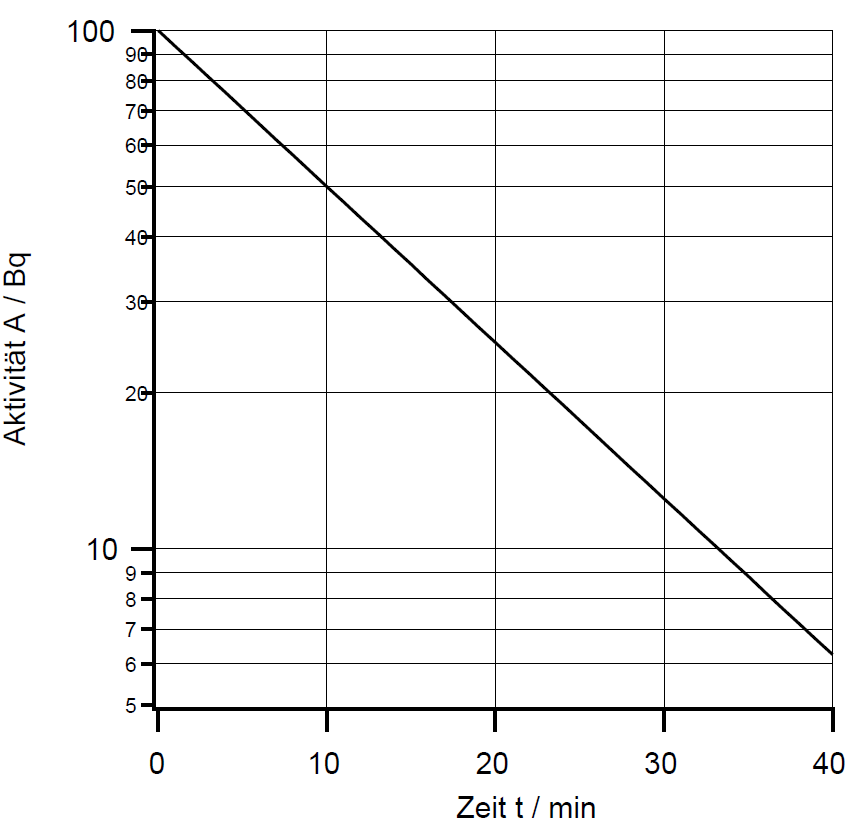
\includegraphics[width=0.5\textwidth]{../../../questions/K/images/zerfallsgesetz.png}

\begin{choices}
	\choice etwa 100 min
	\choice etwa 5 min
	\choice etwa 1 min
	\choice etwa 20 min
	\choice etwa 10 min
\end{choices}

\vspace{3mm}\question Die Halbwertsdicke für Blei bei 100 kV Röntgenstrahlung beträgt ca. 0,012 cm. Sie assistieren bei einer Angiographie mit 100 kV Röntgenstrahlung und tragen eine Bleischürze mit einer Dicke von 0,36 mm Blei. Wieviel Prozent der Strahlung wird abgeschirmt?

\begin{choices}
	\choice 75 %
	\choice 67 %
	\choice 93,5 %
	\choice 87,5 %
	\choice 12,5 %
\end{choices}

\vspace{3mm}\question Was hat keinen Einfluss auf die gemessene Zählrate?

\begin{choices}
	\choice Aktivität der Quelle
	\choice Absorbermaterial
	\choice Abstand zur Quelle
	\choice Absorberdicke
	\choice Temperatur
\end{choices}

\vspace{3mm}\question Welche Strahlungsart hat die kleinste Reichweite in Materie (bei gleicher Energie)?

\begin{choices}
	\choice \( \beta^+ \)-Strahlung
	\choice alpha-Strahlung
	\choice Röntgenstrahlung
	\choice gamma-Strahlung
	\choice \( \beta^- \)-Strahlung
\end{choices}

\vspace{3mm}\end{questions}

\end{document}
